\documentclass{beamer}
%
% Choose how your presentation looks.
%
% For more themes, color themes and font themes, see:
% http://deic.uab.es/~iblanes/beamer_gallery/index_by_theme.html
%
\mode<presentation>
{
  \usetheme{Madrid}      % or try Darmstadt, Madrid, Warsaw, ...
  \usecolortheme{beaver} % or try albatross, beaver, crane, ...
  \usefonttheme{serif}  % or try serif, structurebold, ...
  \setbeamertemplate{navigation symbols}{}
  \setbeamertemplate{caption}[numbered]
} 

\usepackage[english]{babel}
\usepackage[utf8x]{inputenc}
\usepackage{xcolor}
\usepackage{listings}
\lstset
{
    language=[LaTeX]TeX,
    breaklines=true,
    basicstyle=\tt\scriptsize,
    %commentstyle=\color{green}
    keywordstyle=\color{blue},
    %stringstyle=\color{black}
    identifierstyle=\color{magenta},
}

\title[Lingüística de corpus]{Lingüística de corpus}
\author{Max Carey}
\institute[UNAM]{Introducción a la lingüística aplicada
\newline
\textit{``You shall know a word by the company it keeps"}
\newline
- J.R. Firth (1957:11)}
\date{23 de octubre de 2017}

\AtBeginSection[]
{
  \begin{frame}<beamer>
    \frametitle{Outline}
    \tableofcontents[currentsection,currentsubsection]
  \end{frame}
}

\begin{document}

\begin{frame}
  \titlepage
\end{frame}

% Uncomment these lines for an automatically generated outline.
\begin{frame}{Outline}
  \tableofcontents
\end{frame}

\section{Antecedentes históricas}

\begin{frame}{Antecedentes históricas}
	\begin{columns}
    	\begin{column}{6cm}
        	\begin{figure}
    		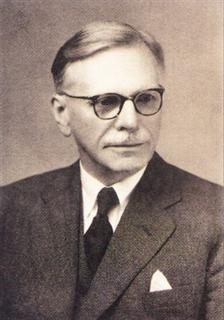
\includegraphics[height=1.8cm]{firth.png}
       		\end{figure}
            \begin{center}
				\tiny
				J.R. Firth \\
				Lingüísta inglés \\
				1890-1960\\
			\end{center}
       		\begin{figure}
           		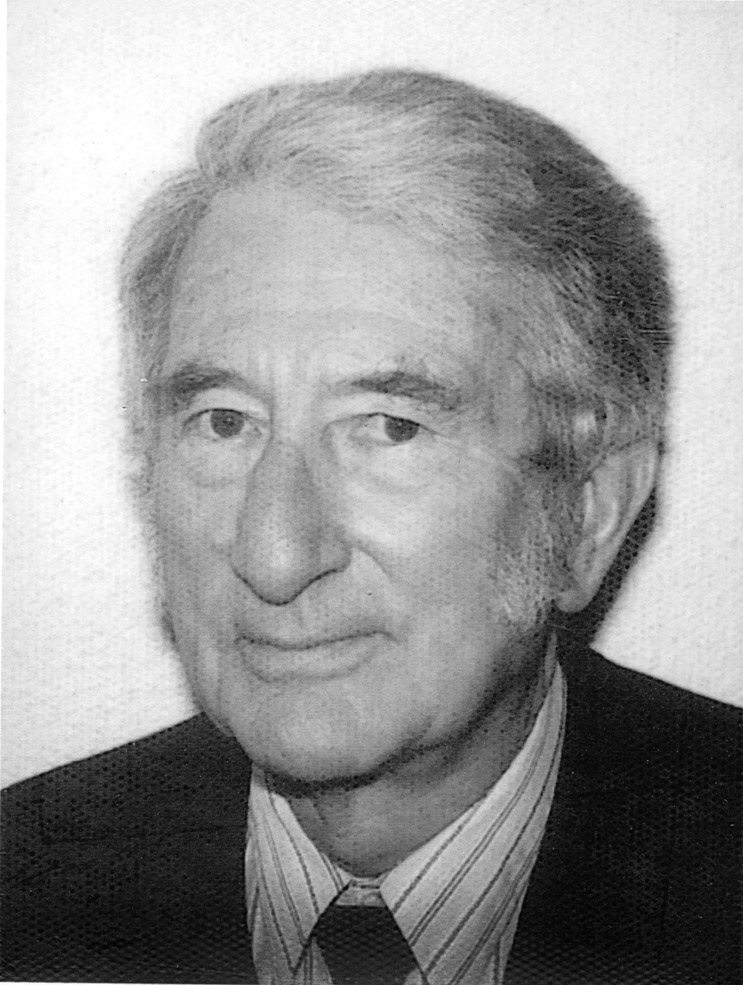
\includegraphics[height=1.8cm]{halliday.jpg}
			\end{figure}
            \begin{center}
				\tiny
				Michael Halliday \\
				Fundador de la gramática sistémico funcional \\
				1925-\\
			\end{center}
        \end{column}
        \begin{column}{6cm}
        	\begin{flushleft}
            \begin{figure}
       	 		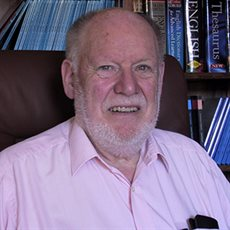
\includegraphics[height=1.8cm]{sinclair.jpg}
        	\end{figure}
            \begin{center}
            \tiny
			John McHardy Sinclair \\
			Fundador de la lingüística de corpus \\
			1933-2007\\
            \end{center}
            \end{flushleft}
        \end{column}
    \end{columns}
\end{frame}


\begin{frame}{J.R. Firth}
	\begin{columns}
    	\begin{column}{6cm}
        	\begin{figure}
    		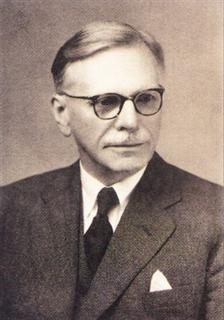
\includegraphics[height=3cm]{firth.png}
       		\end{figure}
            \begin{center}
				\tiny
				J.R. Firth \\
				Lingüísta inglés \\
				1890-1960\\
			\end{center}
        \end{column}
        \begin{column}{6cm}
        	\begin{itemize}
            	\pause
                \item Cabré and Lorente (2003) dicen que es el fundador del funcionalismo lingüístico
                \begin{itemize}
                	\pause
                    \item Incorporó las ideas del antropólogo Mainowski quien dijo: \textit{```el lenguaje no es un sistema en sí mismo (posición estructuralista extrema) sino que evoluciona por las demandas de la sociedad y su contexto'''} (11).
                    \pause
                    \item Creó una definición formal del significado tal que depende del contexto (11).
                \end{itemize}
            \end{itemize}
        \end{column}
    \end{columns}
\end{frame}

\begin{frame}{Sinclair}
	\begin{columns}
    	\begin{column}{6cm}
        	\begin{figure}
    		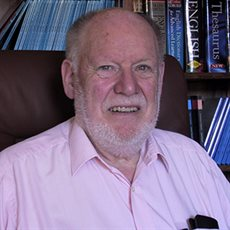
\includegraphics[height=3cm]{sinclair.jpg}
       		\end{figure}
            \begin{center}
			\begin{tiny}
            John McHardy Sinclair \\
			Fundador de la lingüística de corpus \\
			1933-2007\\
            \end{tiny}
			\end{center}
        \end{column}
        \begin{column}{6cm}
        	\begin{itemize}
            	\pause
                \item Fundador del proyecto \textbf{COBUILD} (Collins and Birmingham University International Language Database)
                \begin{itemize}
                	\pause
                    \item Revolucionó la lexicógrafia (Fontenelle 2011: 58)
                \end{itemize}
                \pause
                \item Famoso por dos principios de la lingüística de corpus
                \begin{itemize}
                	\pause
                    \item \textit{the open choice principle}
                    \pause
                    \item \textit{the idiom principle}
                \end{itemize}
            \end{itemize}
        \end{column}
    \end{columns}
\end{frame}

\begin{frame}{The Open Choice Principle}
	\begin{columns}
    	\begin{column}{6cm}
        	\begin{figure}
    			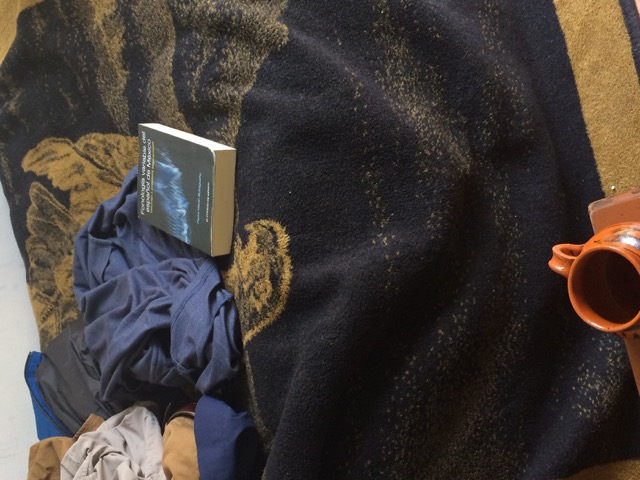
\includegraphics[height=3cm]{pbm.JPG}
            \end{figure}
            	\begin{center}
					\begin{tiny}
            		Fonologia variable del español de México \\
					Pedro Martín Butragueño \\
					2014\\
           			\end{tiny}
				\end{center}
        \end{column}
        \begin{column}{6cm}
        \begin{itemize}
        \item placeholder
        \end{itemize}
        \end{column}
    \end{columns}
\end{frame}



\section{Some History}

\begin{frame}{\TeX{}}
	\begin{columns}
		\begin{column}{4cm}
			\begin{figure}
   				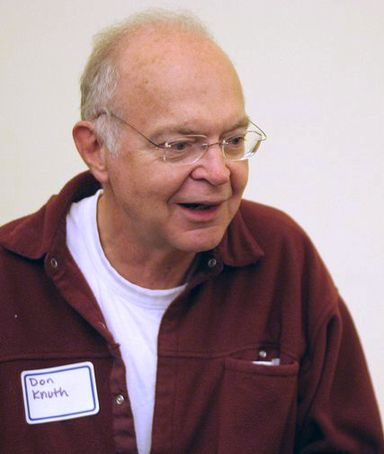
\includegraphics[height=3cm]{384px-KnuthAtOpenContentAlliance.jpg}
   				
\includegraphics[height=3cm]{ArtOfComputerProgramming.jpg}
			\end{figure}
			\begin{center}
				\tiny
				Donald Knuth \\
				Computer Scientist \\
				Born January 10, 1938 (age 77) \\
			\end{center}
		\end{column}
		\begin{column}{6cm}
			\begin{itemize}
				\item \TeX{} was created by Donald Knuth in 1978
				\pause
				\item A typesetting macro language and compiler:
				\begin{itemize}
					\item Readable mathematics
					\item Better hyphenation
					\item Optimized justification
					\item Font management tools
					\item Cross-compatibility
				\end{itemize}
				\pause
				\item Code -- Compile -- Visualize
			\end{itemize}
		\end{column}
	\end{columns}
\end{frame}

\begin{frame}{\LaTeX{}}
\begin{columns}
\begin{column}{4cm}
\begin{figure}
   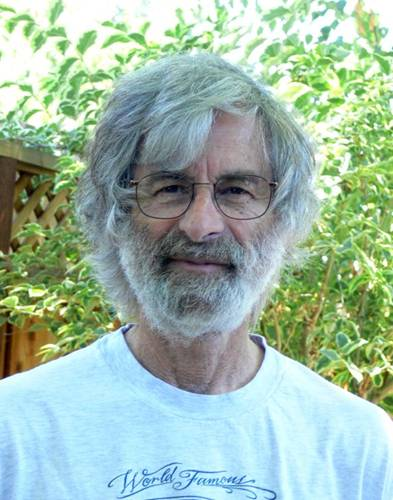
\includegraphics[height=3cm]{leslie.jpg}
   
\includegraphics[height=3cm]{latex.jpg}
\end{figure}
\begin{center}
\tiny
Leslie Lamport \\
Computer Scientist \\
Born February 7, 1941 (age 74) \\
\end{center}
\end{column}
\begin{column}{6cm}
\begin{itemize}
\item \LaTeX{} $=$ Leslie Lamport's \TeX{}
\pause
\item Initial Release in 1984
\pause
\item A macro package for \TeX{} with:
\begin{itemize}
\item Document Types
\item Chapter Headings
\item Footnotes
\item Cross-references
\item Bibliographies
\item Environments (Tables, Figures, Equations)
\end{itemize}
\end{itemize}
\end{column}
\end{columns}
\end{frame}

% \subsection{Tables and Figures}

% \begin{frame}{Tables and Figures}

% \begin{itemize}
% \item Use \texttt{tabular} for basic tables --- see Table~\ref{tab:widgets}, for example.
% \item You can upload a figure (JPEG, PNG or PDF) using the files menu. 
% \item To include it in your document, use the \texttt{includegraphics} command (see the comment below in the source code).
% \end{itemize}

% Commands to include a figure:
%\begin{figure}
%\includegraphics[width=\textwidth]{your-figure's-file-name}
%\caption{\label{fig:your-figure}Caption goes here.}
%\end{figure}

% \begin{table}
% \centering
% \begin{tabular}{l|r}
% Item & Quantity \\\hline
% Widgets & 42 \\
% Gadgets & 13
% \end{tabular}
% \caption{\label{tab:widgets}An example table.}
% \end{table}

% \end{frame}

% \subsection{Mathematics}

% \begin{frame}{Readable Mathematics}

% Let $X_1, X_2, \ldots, X_n$ be a sequence of independent and identically distributed random variables with $\text{E}[X_i] = \mu$ and $\text{Var}[X_i] = \sigma^2 < \infty$, and let
% $$S_n = \frac{X_1 + X_2 + \cdots + X_n}{n}
%       = \frac{1}{n}\sum_{i}^{n} X_i$$
% denote their mean. Then as $n$ approaches infinity, the random variables $\sqrt{n}(S_n - \mu)$ converge in distribution to a normal $\mathcal{N}(0, \sigma^2)$.

% \end{frame}

\section{First Steps}
	
\begin{frame}{Editors and Compilers}
\begin{itemize}
\item To install in your machine
\begin{itemize}
\item Check \texttt{latex-project.org}
\end{itemize}
\pause
\item In the cloud
\begin{itemize}
\item ShareLatex : \texttt{www.sharelatex.com}
\item Overleaf : \texttt{www.overleaf.com}
\end{itemize}
\end{itemize}
\pause
\vskip 1cm
\begin{block}{Please give me Mb of space on Overleaf}
https://www.overleaf.com/signup?ref=d1806010dac8
\end{block}
\end{frame}

\begin{frame}[fragile]{Hello \LaTeX{} World!}
\begin{columns}
\begin{column}{5cm}
\vspace{-2cm}
\lstinputlisting{file1.tex}
\end{column}
\begin{column}{5cm}
Hello \LaTeX{} World!
\end{column}
\end{columns}
\end{frame}

\begin{frame}[fragile]{More structure}
\begin{columns}
\begin{column}{5.5cm}
\lstinputlisting[basicstyle=\sffamily\tiny,]{file2.tex}
\end{column}
\begin{column}{4.5cm}
\vspace{-2cm}
\begin{figure}
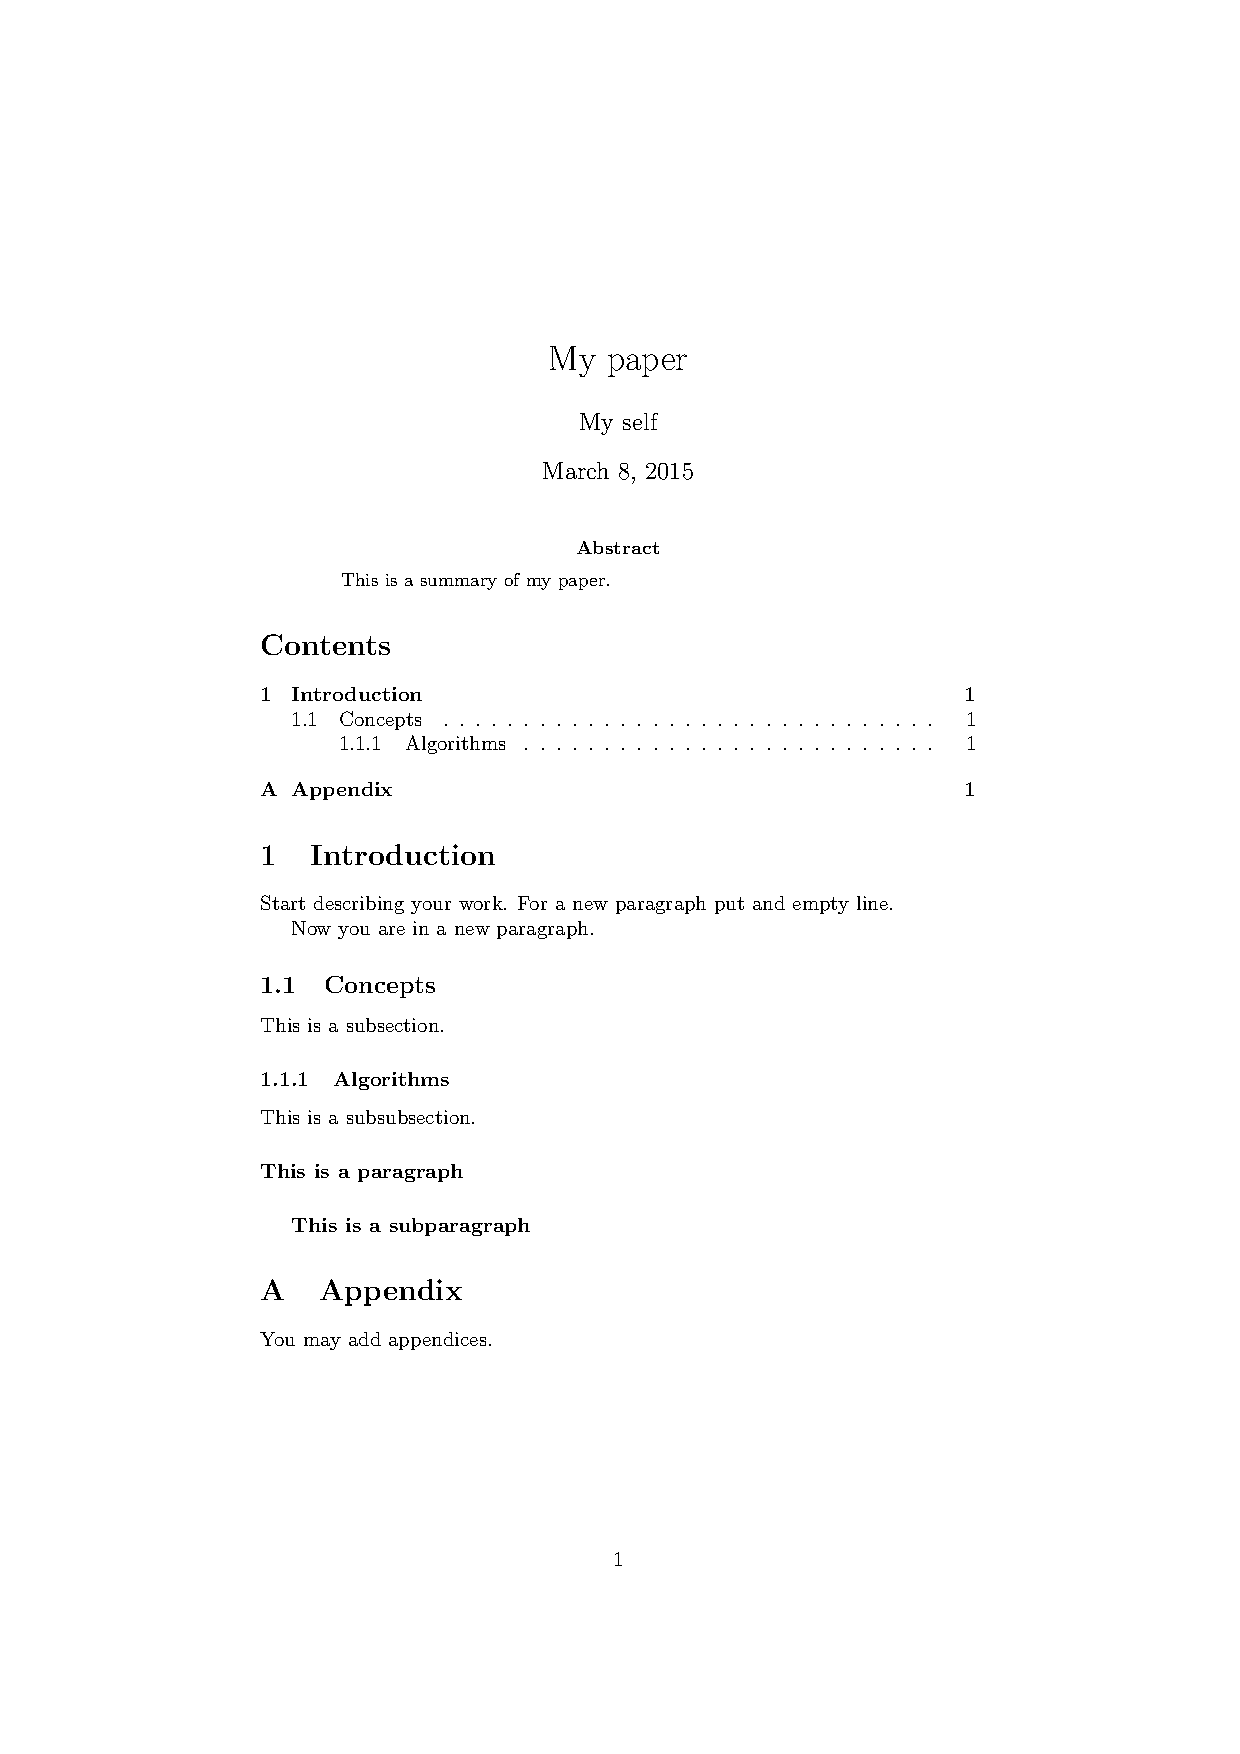
\includegraphics[width=6cm]{file2a.pdf}
\end{figure}
\end{column}
\end{columns}
\end{frame}

\begin{frame}[fragile]{Team work}
\begin{columns}
\begin{column}{5cm}
\lstinputlisting[basicstyle=\sffamily\tiny,]{file3.tex}
\end{column}
\begin{column}{5cm}
\begin{itemize}
\item Using the \texttt{include} macro, each author can work on an independent file. 
\item To compile only a set of files, use the macro \texttt{includeonly}
\item Welcome to team work in \LaTeX{}!
\end{itemize}
\end{column}
\end{columns}
\end{frame}

\section{\LaTeX{} Basics}

	\begin{frame}{LaTeX{} Basics}
		\begin{itemize}
        	\item Documents
        	\item Fonts and Styles
            \item Text Symbols
            \item Paragraphs
            \item Lists
            \item Cross References
            \item Tables
            \item Math Symbols
        	\item Equations
            \item Figures
            \item Bibliography
		\end{itemize}
	\end{frame}

	\begin{frame}{Documents}
    	\begin{columns}
        	\begin{column}{3cm}
              Classes:
              \begin{itemize}
                  \item \texttt{book}
                  \item \texttt{article}
                  \item \texttt{report}
                  \item \texttt{letter}
                  \item \texttt{slides}
                  \item \texttt{beamer}
                  \item \texttt{IEEETran}
                  \item \texttt{minimal}
                  \item \ldots
              \end{itemize}
        	\end{column}
            \begin{column}{7cm}
              Options:
              \begin{itemize}
                  \item \texttt{10pt, 11pt, 12pt}
                  \item \texttt{a4paper, letterpaper,\ldots}
                  \item \texttt{fleqn, leqno}
                  \item \texttt{titlepage, notitlepage}
                  \item \texttt{twocolumn}
                  \item \texttt{twoside, oneside}
                  \item \texttt{landscape}
                  \item \texttt{openright, openany}
                  \item \texttt{draft}
              \end{itemize}
        	\end{column}
    	\end{columns}
	\end{frame}

\begin{frame}[fragile]
\frametitle{Fonts and Styles}
\begin{tabular}[c]{|l l|l l|}
\hline
\verb!\textrm{Hello}! & \textrm{Hello} & \verb!{\tiny Hello}! & {\tiny Hello} \\
\hline
\verb!\textsf{Hello}! & \textsf{Hello} & \verb!{\scriptsize Hello}! & {\scriptsize Hello} \\
\hline
\verb!\texttt{Hello}! & \texttt{Hello} & \verb!{\footnotesize Hello}! & {\footnotesize Hello} \\
\hline
\verb!\textmd{Hello}! & \textmd{Hello} & \verb!{\small Hello}! & {\small Hello} \\
\hline
\verb!\textbf{Hello}! & \textbf{Hello} & \verb!{\normalsize Hello}! & {\normalsize Hello} \\
\hline
\verb!\textup{Hello}! & \textup{Hello} & \verb!{\large Hello}! & {\large Hello} \\
\hline
\verb!\textit{Hello}! & \textit{Hello} & \verb!{\Large Hello}! & {\Large Hello} \\
\hline
\verb!\textsl{Hello}! & \textsl{Hello} & \verb!{\LARGE Hello}! & {\LARGE Hello} \\
\hline
\verb!\underline{Hello}! & \underline{Hello} & \verb!{\huge Hello}! & {\huge Hello} \\
\hline
\verb!\textsc{Hello}! & \textsc{Hello} & \verb!{\Huge Hello}! & {\Huge Hello} \\
\hline
\end{tabular}
\end{frame}
        
\begin{frame}[fragile]
\frametitle{Text Symbols}
\begin{center}
\begin{tabular}[c]{|l l|l l|l l|}
\hline
\verb!\$! & \$ & \verb!``! & ``  & \verb!\oe! & \oe \\
\hline
\verb!\&! & \& & \verb!''! & '' & \verb!\OE! & \OE\\
\hline
\verb!\%! & \% & \verb!"! & " & \verb!\ae! & \ae\\
\hline
\verb!\#! & \# & \verb!\'a! & \'a & \verb!\AE! & \AE\\
\hline
\verb!\S! & \S & \verb!\`a! & \`a & \verb!\o! & \o\\
\hline
\verb!\LaTeX{}! & \LaTeX{} & \verb!\~a! & \~a & \verb!\O! & \O\\
\hline
\verb!A\_B! & A\_B & \verb!\^a! & \^a & \verb!\l! & \l\\
\hline
\verb!\textbar! & \textbar & \verb!\c a! & \c a & \verb!\L! & \L\\
\hline
\verb!\textbullet! & \textbullet & \verb!\"a! & \"a & \verb!\i! & \i\\
\hline
\verb!\textbackslash! & \textbackslash & \verb!\v a! & \v a & \verb!\j! & \j\\
\hline
\verb!\ldots! & \ldots & \verb!\H a! & \H a & \verb!\aa! & \aa\\
\hline
\verb!\~{}! &\~{} & \verb!\=a! & \=a & \verb!\AA! & \AA\\
\hline
\verb!\^{}! &\^{} & \verb!\d a! & \d a & \verb!A-B! & A-B\\
\hline
\verb!\textless! & \textless & \verb!\.a! & \.a & \verb!A--B! & A--B\\
\hline
\verb!\textgreater! & \textgreater & \verb!\b a! & \b a & \verb!A---B! & A---B\\
\hline
\end{tabular} 
\end{center}
\end{frame}

\begin{frame}[fragile]{Paragraphs}
\begin{columns}
\begin{column}{6cm}
\vspace{-0.3cm}
\begin{lstlisting}
\begin{center}
Please give me space on Overleaf
\end{center}
\end{lstlisting}
\begin{lstlisting}
\begin{flushleft}
Please give me space on Overleaf
\end{flushleft}
\end{lstlisting}
\begin{lstlisting}
\begin{flushright}
Please give me space on Overleaf
\end{flushright}
\end{lstlisting}
\begin{lstlisting}
\begin{quote}
Please give me space on Overleaf
\end{quote}
\end{lstlisting}
\begin{lstlisting}
\begin{quotation}
Please give me space on Overleaf
\end{quotation}
\end{lstlisting}
\begin{lstlisting}
\begin{verse}
Please give me space on Overleaf
\end{verse}
\end{lstlisting}
\end{column}
\begin{column}{4cm}
\vspace{-0.5cm}
\footnotesize
\begin{center}
Please give me space on Overleaf
\end{center}
\begin{flushleft}
Please give me space on Overleaf
\end{flushleft}
\begin{flushright}
Please give me space on Overleaf
\end{flushright}
\begin{quote}
Please give me space on Overleaf
\end{quote}
\begin{quotation}
Please give me space on Overleaf
\end{quotation}
\begin{verse}
Please give me space on Overleaf
\end{verse}
\end{column}
\end{columns}
\end{frame}

\begin{frame}[fragile]{Paragraphs}
\begin{columns}
\begin{column}{6cm}
\vspace{-0.3cm}
\begin{lstlisting}
\begin{itemize}
\item One item
\item Another item
\end{itemize}
\end{lstlisting}
\begin{lstlisting}
\begin{enumerate}
\item First item
\item Second item
\end{enumerate}
\end{lstlisting}
\begin{lstlisting}
\begin{description}
\item[Lion] A mammal
\item[Shark] A fish
\end{description}
\end{lstlisting}
\begin{lstlisting}
\begin{itemize}
\item A list inside a list
\begin{enumerate}
\item Lists 
\item can be 
\item recursive
\end{enumerate}
\end{itemize}
\end{lstlisting}
\end{column}
\begin{column}{4cm}
\vspace{-1cm}
\footnotesize
\begin{itemize}
\item One item
\item Another item
\end{itemize}
\vspace{0.5cm}
\begin{enumerate}
\item First item
\item Second item
\end{enumerate}
\vspace{0.5cm}
\begin{description}
\item[Lion] A mammal
\item[Shark] A fish
\end{description}
\vspace{0.5cm}
\begin{itemize}
\item A list inside a list
\begin{enumerate}
\item Lists 
\item can be 
\item recursive
\end{enumerate}
\end{itemize}
\end{column}
\end{columns}
\end{frame}

\begin{frame}[fragile]{Cross References}
\begin{columns}
\begin{column}{6cm}
\begin{itemize}
% \item Numbered items and pages can be referenced anywhere in the text.
% \item Numbered items can be document elements (parts, chapters, sections, subsections), equations, figures, tables, \ldots
\item Use macro \verb!\label{!\textit{some-- identifier}\verb!}! to set a mark.
\item Use macro \verb!\ref{!\textit{some-- identifier}\verb!}! to retrieve the number of the item where the mark is defined.
\item Use macro \verb!\pageref{!\textit{some-- identifier}\verb!}! to retrieve the page number where mark is defined.
\end{itemize}
\begin{lstlisting}
\label{marcador}
This is slide \ref{marcador}. \\
It is in page \pageref{marcador}.
\end{lstlisting}
\end{column}
\begin{column}{4cm}
\label{marcador}
\begin{center}
This is slide \ref{marcador}. \\
It is in page \pageref{marcador}.
\end{center}
\end{column}
\end{columns}
\end{frame}

\begin{frame}[fragile]{Tables}
\begin{lstlisting}
\begin{table}
\begin{tabular}{ l | c | r | p{6cm}}
Name & Age & Height & Email \\
\hline
Alex & 44 & 1,80m & alex@isr.ist.utl.pt \\
\end{tabular}
\caption{JEEC 2015 Monday Workshop Participants}
\end{table}
\end{lstlisting}
\begin{table}
\begin{tabular}{ l | c | r | p{6cm}}
Name & Age & Height & Email \\
\hline
Alex & 44 & 1,80m & alex@isr.ist.utl.pt \\
\end{tabular}
\caption{JEEC 2015 Monday Workshop Participants}
\end{table}
\end{frame}

\begin{frame}[fragile]{Math Symbols}
\begin{columns}
\begin{column}{4.5cm}
\begin{lstlisting}
Equation $E_c=\frac{mv^2}{2}$ is true
\end{lstlisting}

\begin{block}{}
Equation $E_c=\frac{mv^2}{2}$ is true
\end{block}
\vspace{0.5cm}
\begin{lstlisting}
Equation \[E_c=\frac{mv^2}{2}\] is true
\end{lstlisting}

\begin{block}{}
Equation \[E_c=\frac{mv^2}{2}\] is true
\end{block}
\end{column}
\begin{column}{5.5cm}
\begin{center}
\scriptsize
\begin{tabular}{| l l | l l|}
\hline
\verb!\sqrt[n]{x}! & $\sqrt[n]{x}$ & \verb!\alpha! & $\alpha$
\\
\hline
\verb!\sum_{k=1}^N! & $\sum_{k=1}^N$ & \verb!\beta! & $\beta$
\\
\hline
\verb!\int_{k=1}^N! & $\int_{k=1}^N$ & \verb!\leq! & $\leq$
\\
\hline
\verb!\prod_{k=1}^N! & $\prod_{k=1}^N$ & \verb!\geq! & $\geq$
\\
\hline
\verb!\overbrace{ab}! & $\overbrace{ab}$ & \verb!\infty! & $\infty$
\\
\hline
\verb!\widetilde{ab}! & $\widetilde{ab}$ & \verb!\times! & $\times$
\\
\hline
\verb!\Rightarrow! & $\Rightarrow$ & \verb!\forall! & $\forall$
\\
\hline
\verb!\Updownarrow! & $\Updownarrow$ & \verb!\exists! & $\exists$
\\
\hline
\verb!\tilde{a}! & $\tilde{a}$ & \verb!\in! & $\in$
\\
\hline
\verb!\hat{a}! & $\hat{a}$ & \verb!\pm! & $\pm$
\\
\hline
\verb!\dot{a}! & $\dot{a}$ & \verb!\neq! & $\neq$ \\
\hline
\verb!\ddot{a}! & $\ddot{a}$ & \verb!\mid! & $\mid$
\\
\hline
\verb!\arctan! & $\arctan$ & \verb!\subset! & $\subset$
\\
\hline
\verb!\limsup! & $\limsup$ & \verb!\cup! & $\cup$
\\
\hline
\verb!\bigotimes! & $\bigotimes$ & \verb!\angle! & $\angle$
\\
\hline
\verb!\bigodot! & $\bigodot$ & \verb!\cdots! & $\cdots$
\\
\hline
\verb!\approx! & $\approx$ & \verb!\flat! & $\flat$
\\
\hline
\verb!\doteq! & $\doteq$ & \verb!\Box! & $\Box$
\\
\hline
\verb!\emptyset! & $\emptyset$ & \verb!\partial! & $\partial$
\\
\hline
\end{tabular}
\end{center}
\end{column}
\end{columns}
\end{frame}

\begin{frame}[fragile]{Equations}
The \texttt{equation} environment automatically numbers equations. 

If numbering is not needed use \texttt{equation*}.
\begin{lstlisting}
\begin{equation}
\label{eq:matrix_transpose}
\left[\begin{array}{ccc} a_{11} & \cdots & a_{1n} \\
\vdots & \ddots & \vdots \\ a_{n1} & \cdots & a_{nn}
\end{array}\right]^T= 
\left[\begin{array}{ccc} a_{11} & \cdots & a_{n1} \\
\vdots & \ddots & \vdots \\ a_{1n} & \cdots & a_{nn}
\end{array}\right]
\end{equation}
\end{lstlisting}

\begin{equation}
\label{eq:matrix_transpose}
\left[
\begin{array}{ccc}
a_{11} & \cdots & a_{1n} \\
\vdots & \ddots & \vdots \\
a_{n1} & \cdots & a_{nn}
\end{array}
\right]^T
= 
\left[
\begin{array}{ccc}
a_{11} & \cdots & a_{n1} \\
\vdots & \ddots & \vdots \\
a_{1n} & \cdots & a_{nn}
\end{array}
\right]
\end{equation}
\end{frame}

\begin{frame}[fragile]{Figures}
Graphics files (*.jpg, *.png, *.pdf, etc) can be displayed in a \texttt{figure} environment, using command \verb!\includegraphics! from the \texttt{graphicx} package.
\begin{columns}
\begin{column}{5cm}
\begin{lstlisting}
\usepackage{graphicx}
\begin{figure}[!htpb]
\label{fig:leslie}
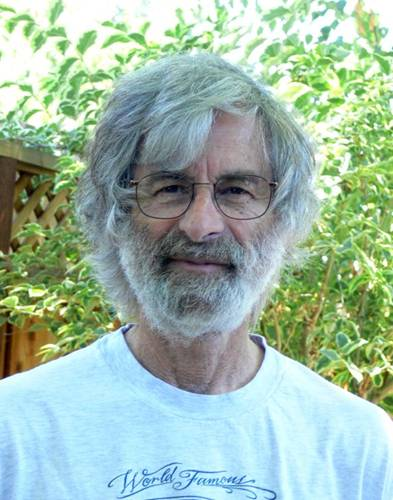
\includegraphics[width=2.5cm]{leslie.jpg}
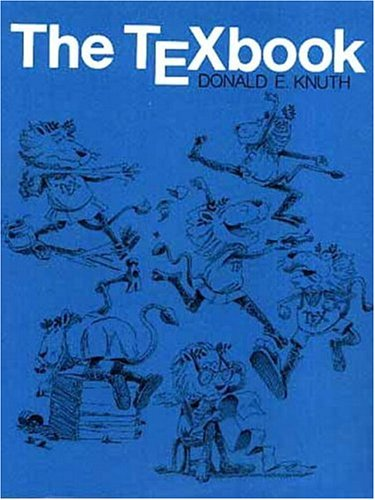
\includegraphics[width=2.5cm]{texbook.jpg}
\caption{Leslie Lamport and his TeXbook.}
\end{figure}
\end{lstlisting}
\end{column}
\begin{column}{5cm}
\begin{figure}[!htpb]
\label{fig:leslie}
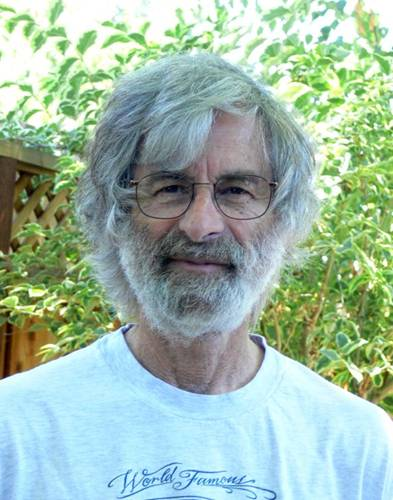
\includegraphics[width=2.5cm]{leslie.jpg}
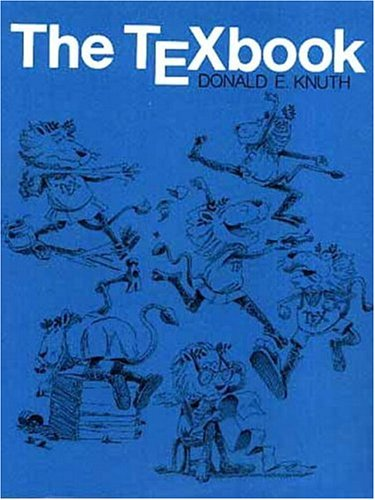
\includegraphics[width=2.5cm]{texbook.jpg}
\caption{Leslie Lamport and his textbook.}
\end{figure}
\end{column}
\end{columns}
\end{frame}

\begin{frame}[fragile]{Bibliography}

Use BibTeX. Put your bibliography in a separate file (e.g. biblio.bib): 
\begin{lstlisting}
@book{lamport86 ,
     author =    "Leslie Lamport" ,
     title =     "\LaTeX: A Document Preparation System" ,
     publisher = "Addison--Wesley Pub.\ Co." ,
     year =      "1986" ,
     address =   "Reading, MA" }
\end{lstlisting}
Now use it in your main file.
\begin{columns}
\begin{column}{5cm}
\begin{lstlisting}
In \cite{lamport86} is given a detailed description of the use of BibTeX.
...
\bibliographystyle{plain}
\bibliography{biblio.bib}
\end{lstlisting}
\end{column}
\begin{column}{5cm}
In \cite{lamport86} is given a detailed description of the use of BibTeX.
\end{column}
\end{columns}
\bibliographystyle{plain}
\bibliography{biblio.bib}
\end{frame}

\section{Conclusion}
	
    \begin{frame}{Conclusion}
		\begin{columns}
			\begin{column}{5cm}
				\begin{figure}
   					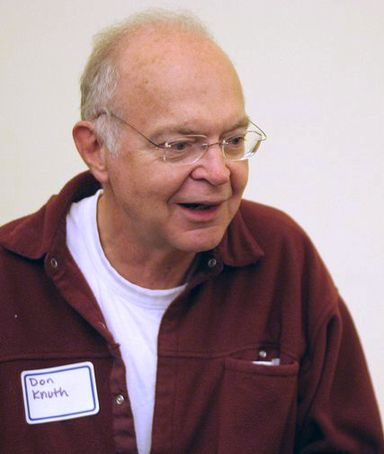
\includegraphics[height=4cm]{384px-KnuthAtOpenContentAlliance.jpg}
				\end{figure}
			\end{column}
			\begin{column}{5cm}
				\begin{flushright}
					\textit{The ideal situation occurs when
the things that we regard as beautiful
are also regarded by other
people as useful.}
					\vskip 0.5cm
				-- Donald Knuth
				\end{flushright}
			\end{column}
		\end{columns}
	\end{frame}

\end{document}
